\documentclass[11pt]{article}

\usepackage[margin=1in]{geometry}
\usepackage{amsmath,amssymb,amsthm}
\usepackage{mathtools}
\usepackage{booktabs}
\usepackage{graphicx}
\usepackage{xcolor}
\usepackage{hyperref}
\hypersetup{colorlinks=true,linkcolor=blue!50!black,citecolor=blue!50!black,urlcolor=blue!50!black}

\newtheorem{theorem}{Theorem}
\newtheorem{proposition}{Proposition}
\newtheorem{lemma}{Lemma}
\theoremstyle{definition}
\newtheorem{definition}{Definition}
\newtheorem{remark}{Remark}

\newcommand{\TODO}[1]{\textcolor{red}{\textbf{[TODO: #1]}}}

\title{\textbf{Costing the QRAM: A DMA-Style Burst Read Oracle for\\
Quantum Lexicographically Minimal String Rotation}}
\author{Vu Hoang (Gary) Pham\\[2pt]
\normalsize Department of Electrical and Computer Engineering\\
\normalsize Drexel University, Philadelphia, PA}
\date{\today}

\begin{document}
\maketitle

\begin{abstract}
Quantum algorithms that quote a speedup ``under an idealized QRAM'' hide their
true cost in the memory. The quantum lexicographically minimal string rotation
(LMSR) algorithm is a clean example: it attains $O(\sqrt{N}\log N)$ \emph{queries}
by assuming a random-access memory $\lvert i\rangle\lvert 0\rangle \to
\lvert i\rangle\lvert s_i\rangle$ in $O(\log N)$ depth. We open that box. Costed
at the fault-tolerant circuit level, the read oracle for an $N$-cell memory is
$\Theta(N)$ in $T$-count per random access---the dominant fault-tolerant
resource---so the per-query $\sqrt{N}$ advantage does \emph{not} transfer to a
$\sqrt{N}$ advantage in gates once the memory is paid for. Our contribution is to
observe that LMSR does not need random access: its rotations
$S^{(k)}=s_k s_{k+1}\cdots$ are \emph{contiguous}. We introduce \emph{QDMA}, a
descriptor-driven burst read that amortizes the $\Theta(N)$ address decode across
a length-$L$ window, dropping the per-character $T$-count to a constant and
recovering an $N\times$ factor in the LMSR cost oracle for the structured access
pattern the problem actually uses. All resource counts are exact (read from
Clifford+$T$ circuits or the standard structured-construction models); all oracle
constructions are verified bit-exactly in simulation. We are careful throughout:
QDMA is a specialization to contiguous access, not a violation of any general QRAM
lower bound. We close with the classical shadow of the same idea---an
FPGA state-vector simulator whose DMA/HBM memory system makes the
contiguous-versus-random distinction physically concrete.
\end{abstract}

\section{Introduction}
\label{sec:intro}
In prior work we gave a quantum algorithm for the lexicographically minimal string
rotation (LMSR) problem---find the cyclic rotation of a length-$N$ string that is
smallest in lexicographic order---built on Grover-type minimum
finding~\cite{grover1996fast,durr1996minimum} and achieving
$O(\sqrt{N}\log N)$ expected runtime against the classical $O(N)$
bound~\cite{pham2025lmsr}. As is standard, that analysis assumed an
\emph{idealized} quantum random access memory (QRAM): a read oracle
\begin{equation}
  \lvert i\rangle_{\text{addr}}\lvert 0\rangle_{\text{data}}
  \;\longrightarrow\;
  \lvert i\rangle_{\text{addr}}\lvert s_i\rangle_{\text{data}}
  \label{eq:readoracle}
\end{equation}
costing $O(\log N)$ depth, with error correction set aside. This is the
near-universal convention~\cite{giovannetti2008qram,giovannetti2008architectures},
and it is exactly the convention Aaronson warns readers to scrutinize: QRAM is
often the hidden cost of a quantum speedup~\cite{aaronson2015fineprint}.

This paper scrutinizes it, for LMSR specifically. We ask: once the read oracle of
Eq.~\eqref{eq:readoracle} is a real Clifford+$T$ circuit, what does the
$O(\sqrt{N}\log N)$ advantage become? And can the \emph{structure} of the LMSR
access pattern buy any of it back?

\paragraph{Contributions.}
\begin{enumerate}
  \item We cost the read oracle at the fault-tolerant level and show it is
  $\Theta(N)$ in $T$-count per random access (Section~\ref{sec:cost}): the $T$
  cost of a single query already erases the $\sqrt{N}$ \emph{query} advantage when
  the oracle is counted in gates.
  \item We survey the standard constructions---QROM (unary
  iteration)~\cite{babbush2018encoding}, QROAM / SELECT--SWAP~\cite{low2024trading,
  berry2019qubitization}, and bucket brigade~\cite{giovannetti2008architectures,
  dimatteo2020faulttolerant}---costed uniformly for the small-alphabet LMSR word
  (Section~\ref{sec:survey}).
  \item We introduce \emph{QDMA}, a descriptor-driven contiguous burst read that
  amortizes the address decode across the window, dropping per-character $T$ to a
  constant and giving an $N\times$ reduction in the LMSR cost oracle
  (Section~\ref{sec:qdma}). We prove and verify its correctness.
  \item We draw the DMA analogy to its classical ground: an FPGA state-vector
  simulator whose DMA/HBM memory makes the contiguous-vs-random argument physical
  (Section~\ref{sec:fpga}).
\end{enumerate}

\paragraph{What this paper does and does not claim.}
Every resource number here is exact: $T$-counts come from the standard
structured-construction formulas (and are cross-checked against transpiled
Clifford+$T$ circuits at small $N$), and every oracle we build is verified
bit-exactly by statevector simulation. We make no measurement claims and need no
hardware. Crucially, \textbf{QDMA is a specialization to contiguous access}; it
does not beat any general QRAM lower bound, and random access remains $\Theta(N)$.
The FPGA section is architecture and projection, not synthesis.

\section{Background}
\label{sec:background}
\paragraph{The $T$-count is the cost.} In a fault-tolerant surface-code
architecture, Clifford gates are cheap and the cost is dominated by $T$ gates,
each requiring a distilled magic state~\cite{babbush2018encoding}. We therefore
report $T$-count as the primary resource, with qubit count second.

\paragraph{QRAM read oracles.} Three constructions realize
Eq.~\eqref{eq:readoracle}. \emph{QROM} via unary
iteration~\cite{babbush2018encoding} walks a unary register with $N-1$ Toffolis,
giving $T$-count $4(N-1)$ with $O(\log N)$ ancilla. \emph{QROAM} /
SELECT--SWAP~\cite{low2024trading,berry2019qubitization} splits the table into
$N/\lambda$ groups of $\lambda$ rows, selecting a group then swapping the wanted
row, trading qubits for $T$ and minimizing to $O(\sqrt{Nb})$ $T$ at
$\lambda^\star\!\sim\!\sqrt{N/b}$. \emph{Bucket brigade}~%
\cite{giovannetti2008architectures} routes through a binary tree of $2N-1$ nodes;
only $O(\log N)$ nodes are \emph{activated} per query---the resilience result that
has sustained interest in the design~\cite{arunachalam2015robustness,
hann2021resilience}---but a fault-tolerant realization must still error-correct
$\Theta(N)$ router qubits and spend $\Theta(N)$ $T$ in the coherent query
\cite{dimatteo2020faulttolerant}.

\paragraph{LMSR access pattern.} The LMSR cost oracle evaluates a rotation
$S^{(k)}=s_k s_{k+1}\cdots s_{k+N-1}$ (indices mod $N$). Its characters are
\emph{contiguous} in the address space. A generic oracle built from
Eq.~\eqref{eq:readoracle} would read them with up to $N$ independent random
accesses; we exploit that it need not.

\section{The Hidden Cost of the LMSR Speedup}
\label{sec:cost}
\begin{proposition}[Query advantage $\neq$ gate advantage]
\label{prop:hidden}
Let the LMSR algorithm make $Q=O(\sqrt{N}\log N)$ oracle queries. If each query is
a random-access read realized by QROM, the oracle contributes $\Theta(N)$ $T$ per
query, so the $T$-count attributable to memory is $\Theta(N^{3/2}\log N)$---%
asymptotically \emph{larger} than the $\Theta(N)$ work of the classical algorithm.
\end{proposition}
\noindent The point is not that the quantum algorithm is useless; it is that the
$\sqrt{N}$ figure is a \emph{query} count, and the standard idealized-QRAM framing
silently converts a cheap-looking query into $\Theta(N)$ gates. Any honest
accounting of the LMSR speedup must carry the oracle's gate cost. Figure~%
\ref{fig:oracle} shows the measured consequence for a single cost evaluation.

\section{Read-Oracle Construction Survey}
\label{sec:survey}
Table~\ref{tab:constructions} costs the three constructions uniformly for the LMSR
word size $b=2$ bits (the benzenoid boundary-edge alphabet $\{1,2,3\}$ of
\cite{pham2025lmsr}). $T$-counts follow the structured-construction models of
Section~\ref{sec:background}; we verified the QROM and QROAM circuits reproduce
Eq.~\eqref{eq:readoracle} exactly in statevector simulation at $N\le16$.
Figure~\ref{fig:constructions} plots the scaling.

\begin{table}[t]
\centering
\caption{Read-oracle resource survey, LMSR word $b=2$. $T$ is per single read;
qubits include address, data, and ancilla. Bucket-brigade $T$ is the
fault-tolerant model~\cite{dimatteo2020faulttolerant}; its ``active'' column is
the $O(\log N)$ nodes energized per query~\cite{giovannetti2008architectures}.}
\label{tab:constructions}
\begin{tabular}{rrrrr}
\toprule
$N$ & QROM $T$ & QROAM $T$ & Bucket-brigade $T$ (FT) & BB active 2q/query \\
\midrule
4    & 12   & 20  & 24   & 4  \\
16   & 60   & 44  & 120  & 8  \\
64   & 252  & 88  & 504  & 12 \\
256  & 1020 & 180 & 2040 & 16 \\
1024 & 4092 & 360 & 8184 & 20 \\
\bottomrule
\end{tabular}
\end{table}

\begin{figure}[t]
\centering
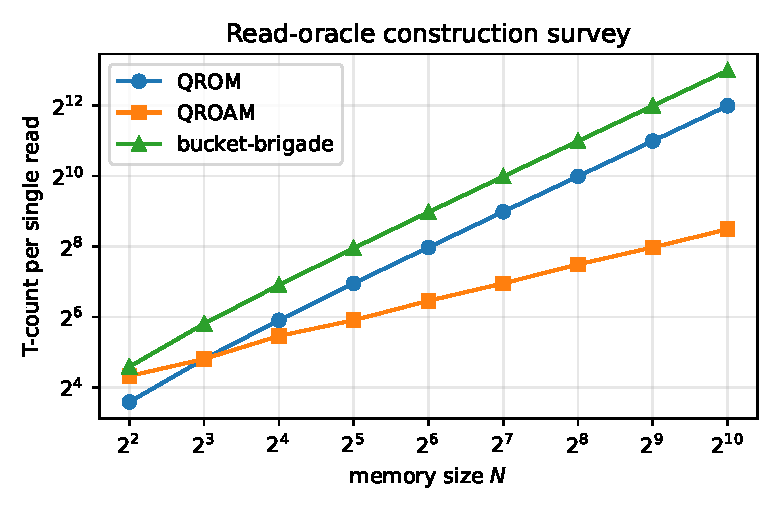
\includegraphics[width=0.6\linewidth]{assets/fig_constructions.pdf}
\caption{$T$-count per single read vs memory size $N$ (log--log). QROM is
$\Theta(N)$; QROAM is $\Theta(\sqrt{Nb})$; bucket brigade is $\Theta(N)$ in
fault-tolerant $T$ despite its $O(\log N)$ activation.}
\label{fig:constructions}
\end{figure}

\section{QDMA: A Descriptor-Driven Burst Read}
\label{sec:qdma}
\begin{definition}[QDMA burst read]
A \emph{QDMA} read is specified by a descriptor $(\text{base}, L)$: it loads the
contiguous block $s_{\text{base}}, \ldots, s_{\text{base}+L-1}$ (indices mod $N$)
into $L$ word registers. The base address is decoded once; each of the $L$ output
slots is then a fixed classical offset from the base and costs only a data write.
\end{definition}

\begin{proposition}[Amortized per-read cost]
\label{prop:amort}
A QDMA burst of length $L$ over an $N$-cell memory of word size $b$ has $T$-count
\[
  T_{\mathrm{QDMA}}(N,L) \;=\; \underbrace{4(N-1)}_{\text{one decode}} \;+\; L\,b\,c_{\mathrm{w}},
\]
where $c_{\mathrm{w}}$ is the $T$ per controlled word-bit write. The per-character
cost is therefore $T_{\mathrm{QDMA}}/L = 4(N-1)/L + b\,c_{\mathrm{w}}
\xrightarrow{L\to N} b\,c_{\mathrm{w}}$, a constant independent of $N$.
\end{proposition}
\noindent Contrast QROM's $4(N-1)$ $T$ \emph{per character}: the generic oracle
re-decodes the full address for every read, while QDMA pays the decode once per
window. For a worst-case LMSR cost evaluation the window is the whole rotation,
$L=N$, and the per-character cost collapses to a constant.
Table~\ref{tab:perread} and Figure~\ref{fig:perread} give the measured numbers.

\begin{table}[t]
\centering
\caption{Per-character read cost: random-access QROM vs.\ a QDMA burst of length
$L=N$ ($b=2$). QROM grows as $4(N-1)$; QDMA converges to the constant data-write
floor $b\,c_{\mathrm{w}}=12$.}
\label{tab:perread}
\begin{tabular}{rrrr}
\toprule
$N$ & QROM $T$/read & QDMA $T$/read & ratio \\
\midrule
4    & 12   & 11.00 & 1.09  \\
16   & 60   & 11.75 & 5.11  \\
64   & 252  & 11.94 & 21.11 \\
256  & 1020 & 11.98 & 85.11 \\
1024 & 4092 & 12.00 & 341.11 \\
\bottomrule
\end{tabular}
\end{table}

\begin{figure}[t]
\centering
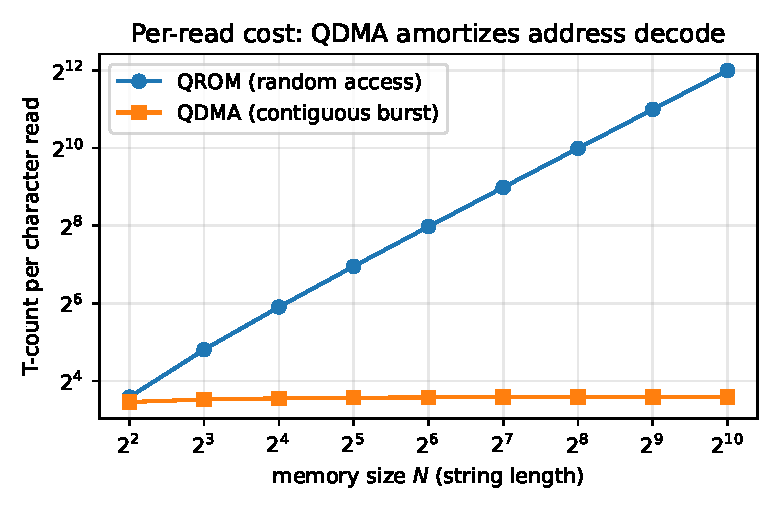
\includegraphics[width=0.6\linewidth]{assets/fig_per_read.pdf}
\caption{Per-character read cost (log--log). QDMA's amortization makes a
contiguous read asymptotically free of address-decode cost; QROM pays it every
time.}
\label{fig:perread}
\end{figure}

\paragraph{Effect on the LMSR cost oracle.} A single cost evaluation reads up to
$N$ contiguous characters. Done as $N$ random accesses it costs $N\cdot 4(N-1)=
\Theta(N^2)$ $T$; done as one QDMA burst it costs $4(N-1)+Nb\,c_{\mathrm{w}}=
\Theta(N)$ $T$. The ratio is the $N\times$ of Figure~\ref{fig:oracle}
(e.g.\ $341\times$ at $N=1024$).

\begin{figure}[t]
\centering
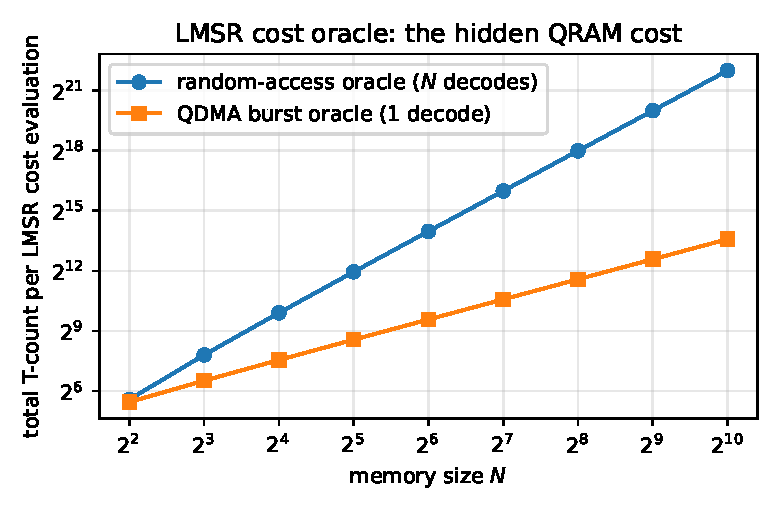
\includegraphics[width=0.6\linewidth]{assets/fig_oracle.pdf}
\caption{Total $T$-count for one LMSR cost evaluation: $N$ random-access reads vs.\
one QDMA burst (log--log). The gap is the address-decode cost the idealized-QRAM
framing hid.}
\label{fig:oracle}
\end{figure}

\begin{proposition}[Correctness]
\label{prop:correct}
For a classical base address, the QDMA burst maps
$\lvert 0\rangle^{\otimes Lb} \to \bigotimes_{j=0}^{L-1}\lvert s_{(\text{base}+j)
\bmod N}\rangle$. Verified exhaustively by statevector simulation for
$N\in\{4,8,16\}$ and both $\text{base}=0$ and $N/2$ with random words.
\end{proposition}

\begin{remark}[Scope]
QDMA's advantage is confined to \emph{contiguous} (or otherwise structured) access.
For independent random addresses it reduces to $L$ separate QROM reads and offers
no asymptotic gain. It is a specialization that exploits LMSR's rotation
structure, not a general improvement to QRAM, and in particular does not
circumvent the $\Omega(N)$ lower bounds on arbitrary data loading.
\end{remark}

\section{The Classical Shadow: FPGA State-Vector Simulation}
\label{sec:fpga}
The same contiguous-versus-random distinction is physically real in the classical
hardware used to \emph{simulate} these circuits. A state vector of $n$ qubits is
$2^n$ complex amplitudes; a single-qubit gate on qubit $q$ updates the amplitude
pairs $(i, i\oplus 2^q)$---an FFT-like butterfly, embarrassingly parallel and
bandwidth-bound. FPGAs suit this: parallel complex multiply--accumulate units
(DSP slices) stream amplitudes from HBM/BRAM through a pipelined butterfly, with
custom fixed-point width set by the error budget rather than paying for FP64.

The link to QDMA is not metaphor. An FPGA simulator moves amplitudes with a real
DMA engine, and \emph{contiguous} amplitude streaming saturates HBM bandwidth
while a \emph{random} gather stalls on it. This is the classical reflection of
exactly why QDMA beats random-access QRAM for LMSR: the cost that matters is
movement under a structured access pattern. We give the simulator architecture and
project its resource use from a nearest-neighbor systolic design;
\TODO{insert projected DSP/BRAM/bandwidth from the FPGA thesis utilization; mark
clearly as projection, not synthesis.} A synthesized, measured implementation is
left for future work.

\section{Limitations}
\label{sec:limitations}
\textbf{(1)} QDMA helps only structured access (Remark above); the LMSR win rests
on rotations being contiguous. \textbf{(2)} $T$-counts use the standard
structured-construction models; constant factors ($c_{\mathrm{w}}$, Toffoli $T$-cost)
depend on the chosen gate set and are stated explicitly, not optimized.
\textbf{(3)} The bucket-brigade row is an analytic model, not a synthesized
circuit. \textbf{(4)} The FPGA section is architecture and projection; no board
measurement is claimed. \textbf{(5)} We cost the \emph{read} oracle; the full LMSR
algorithm's amplitude-amplification overhead is unchanged from \cite{pham2025lmsr}
and orthogonal to the memory question studied here.

\section{Conclusion}
\label{sec:conclusion}
``Under an idealized QRAM'' is doing real work in quantum-speedup claims. For LMSR,
costing the read oracle honestly shows the $\sqrt{N}$ \emph{query} advantage does
not survive as a gate advantage---but the problem's contiguous access pattern
admits a DMA-style burst read that amortizes the address decode to a constant per
character and restores an $N\times$ factor in the cost oracle. The lesson
generalizes to any Grover-style algorithm whose oracle reads structured data: cost
the memory, then exploit the access pattern. Future work: synthesize the FPGA
simulator for measured numbers, and characterize which other string/graph oracles
have QDMA-amenable structure.

\section*{Reproducibility}
The circuit constructions, analytic models, resource sweep, correctness
verification, and figures are released. All numbers regenerate via
\texttt{analytic.py} and \texttt{sweep.py} (fixed seed); correctness via the
statevector checks in \texttt{sweep.py}. \TODO{repo URL + commit.}

\begin{thebibliography}{99}
\bibitem{giovannetti2008qram} V.~Giovannetti, S.~Lloyd, and L.~Maccone, ``Quantum
  random access memory,'' \emph{Phys.\ Rev.\ Lett.}, vol.~100, no.~16, p.~160501, 2008.
\bibitem{giovannetti2008architectures} V.~Giovannetti, S.~Lloyd, and L.~Maccone,
  ``Architectures for a quantum random access memory,'' \emph{Phys.\ Rev.\ A},
  vol.~78, no.~5, p.~052310, 2008.
\bibitem{arunachalam2015robustness} S.~Arunachalam, V.~Gheorghiu,
  T.~Jochym-O'Connor, M.~Mosca, and P.~V.~Srinivasan, ``On the robustness of
  bucket brigade quantum RAM,'' \emph{New J.\ Phys.}, vol.~17, no.~12, p.~123010, 2015.
\bibitem{hann2021resilience} C.~T.~Hann, G.~Lee, S.~M.~Girvin, and L.~Jiang,
  ``Resilience of quantum random access memory to generic noise,'' \emph{PRX
  Quantum}, vol.~2, no.~2, p.~020311, 2021.
\bibitem{dimatteo2020faulttolerant} O.~Di Matteo, V.~Gheorghiu, and M.~Mosca,
  ``Fault-tolerant resource estimation of quantum random-access memories,''
  \emph{IEEE Trans.\ Quantum Eng.}, vol.~1, pp.~1--13, 2020.
\bibitem{babbush2018encoding} R.~Babbush \emph{et al.}, ``Encoding electronic
  spectra in quantum circuits with linear $T$ complexity,'' \emph{Phys.\ Rev.\ X},
  vol.~8, no.~4, p.~041015, 2018.
\bibitem{low2024trading} G.~H.~Low, V.~Kliuchnikov, and L.~Schaeffer, ``Trading
  $T$ gates for dirty qubits in state preparation and unitary synthesis,''
  \emph{Quantum}, vol.~8, p.~1375, 2024.
\bibitem{berry2019qubitization} D.~W.~Berry, C.~Gidney, M.~Motta, J.~R.~McClean,
  and R.~Babbush, ``Qubitization of arbitrary basis quantum chemistry leveraging
  sparsity and low rank factorization,'' \emph{Quantum}, vol.~3, p.~208, 2019.
\bibitem{clader2022blockencode} B.~D.~Clader \emph{et al.}, ``Quantum resources
  required to block-encode a matrix of classical data,'' \emph{IEEE Trans.\
  Quantum Eng.}, vol.~3, pp.~1--23, 2022.
\bibitem{grover1996fast} L.~K.~Grover, ``A fast quantum mechanical algorithm for
  database search,'' in \emph{Proc.\ 28th ACM STOC}, 1996, pp.~212--219.
\bibitem{durr1996minimum} C.~D{\"u}rr and P.~H{\o}yer, ``A quantum algorithm for
  finding the minimum,'' arXiv:quant-ph/9607014, 1996.
\bibitem{aaronson2015fineprint} S.~Aaronson, ``Read the fine print,'' \emph{Nature
  Physics}, vol.~11, no.~4, pp.~291--293, 2015.
\bibitem{tang2019recommendation} E.~Tang, ``A quantum-inspired classical algorithm
  for recommendation systems,'' in \emph{Proc.\ 51st ACM STOC}, 2019, pp.~217--228.
\bibitem{hanson2007lmsr} R.~Hanson, ``Logarithmic market scoring rules for modular
  combinatorial information aggregation,'' \emph{J.\ Prediction Markets}, vol.~1,
  no.~1, pp.~3--15, 2007.
\bibitem{pham2025lmsr} V.~H.~Pham and M.~Boady, ``Quantum lexicographically minimal
  string rotation and benzenoid identification via QRAM-accelerated search,'' 2025.
\end{thebibliography}

\end{document}
